\section{Results}\label{sec.results}

We have implemented our prostate cancer progression model in the dReach's modeling language. The model files are available at \url{http://www.cs.cmu.edu/~liubing/hscc15/}. All the experiments reported below were done using a machine with two Intel Xeon E5-2650 2.00GHz processors and 32GB RAM. The precision $\delta$ was set to $10^{-3}$. 

\subsection{CRC proliferation dynamics}
Due to the lack of biomarkers distinguishing HSCs and CRCs \textit{in vivo}, the proliferation kinetics of CRCs in response to androgen is far from known. Three hypotheses, denoted as $H_1$, $H_2$ and $H_3$ have been proposed to describe the androgen-depenent CRC growth \cite{ideta08}, which are discriminated by the value of $d$ in our model, i.e.:
\begin{itemize}
\item $H_1: d = 0$, the grow of CRCs is independent of $z(t)$;
\item $H_2: d = 1-\frac{\beta_y}{\alpha_y}$, CRCs cease growing when $z(t)=z_0$;
\item $H_3: d = 1$, CRCs decrease when $z(t)=z_0$.
\end{itemize} 

The Patient\#1 data presented in Figure 4 shows that with proper treatment schedules, it is possible to avoid his cancer relapse within $7$ years. We now show that only $H_3$ agrees with this observation. As the PSA level $v(t)$ reflects the total number of cancer cells and CRCs are response for recurrent cancer, we use two invariants: $0 \le v(t) \le 30$ and $0 \le y(t) \le 1$ to specify the property of ``no cancer relapse''. We then carried out $\delta$-reachability analysis to verify whether the invariants hold for each of the model candidates within a bounded time of $365$ days. Here the treatment schedule threshold parameters were provided as ranges: $r_0 \in [0, 7.99]$ (ng ml$^{-1}$) and $r_1 \in [8,15]$ (ng ml$^{-1}$).

%fixed as $r_0=4$ (ng ml$^{-1}$) and $r_1=10$ (ng ml$^{-1}$). The range of the initial concentration of androgen was given as $[15, 17]$ (nM).

The $\mathsf{unsat}$ answers were returned for $H_1$ and $H_2$ (Run\#1 and Run\#2, Table \ref{runs}), indicating that they will always lead to cancer relapse no matter which 
%initial androgen concentration 
treatment schedule 
was chosen. In contrast, $\delta$-$\mathsf{sat}$ was returned for $H_3$ (Run\#3, Table \ref{runs}). Witness trajectories are shown in Figure \ref{prostate-fig1}), demonstrating that the cancer relapse can be avoid in a bound time as observed experimentally \cite{ bruchovsky06,bruchovsky07}. The rest of the results in this paper were generated using $H_3$.

\begin{figure}[htb]
\centering
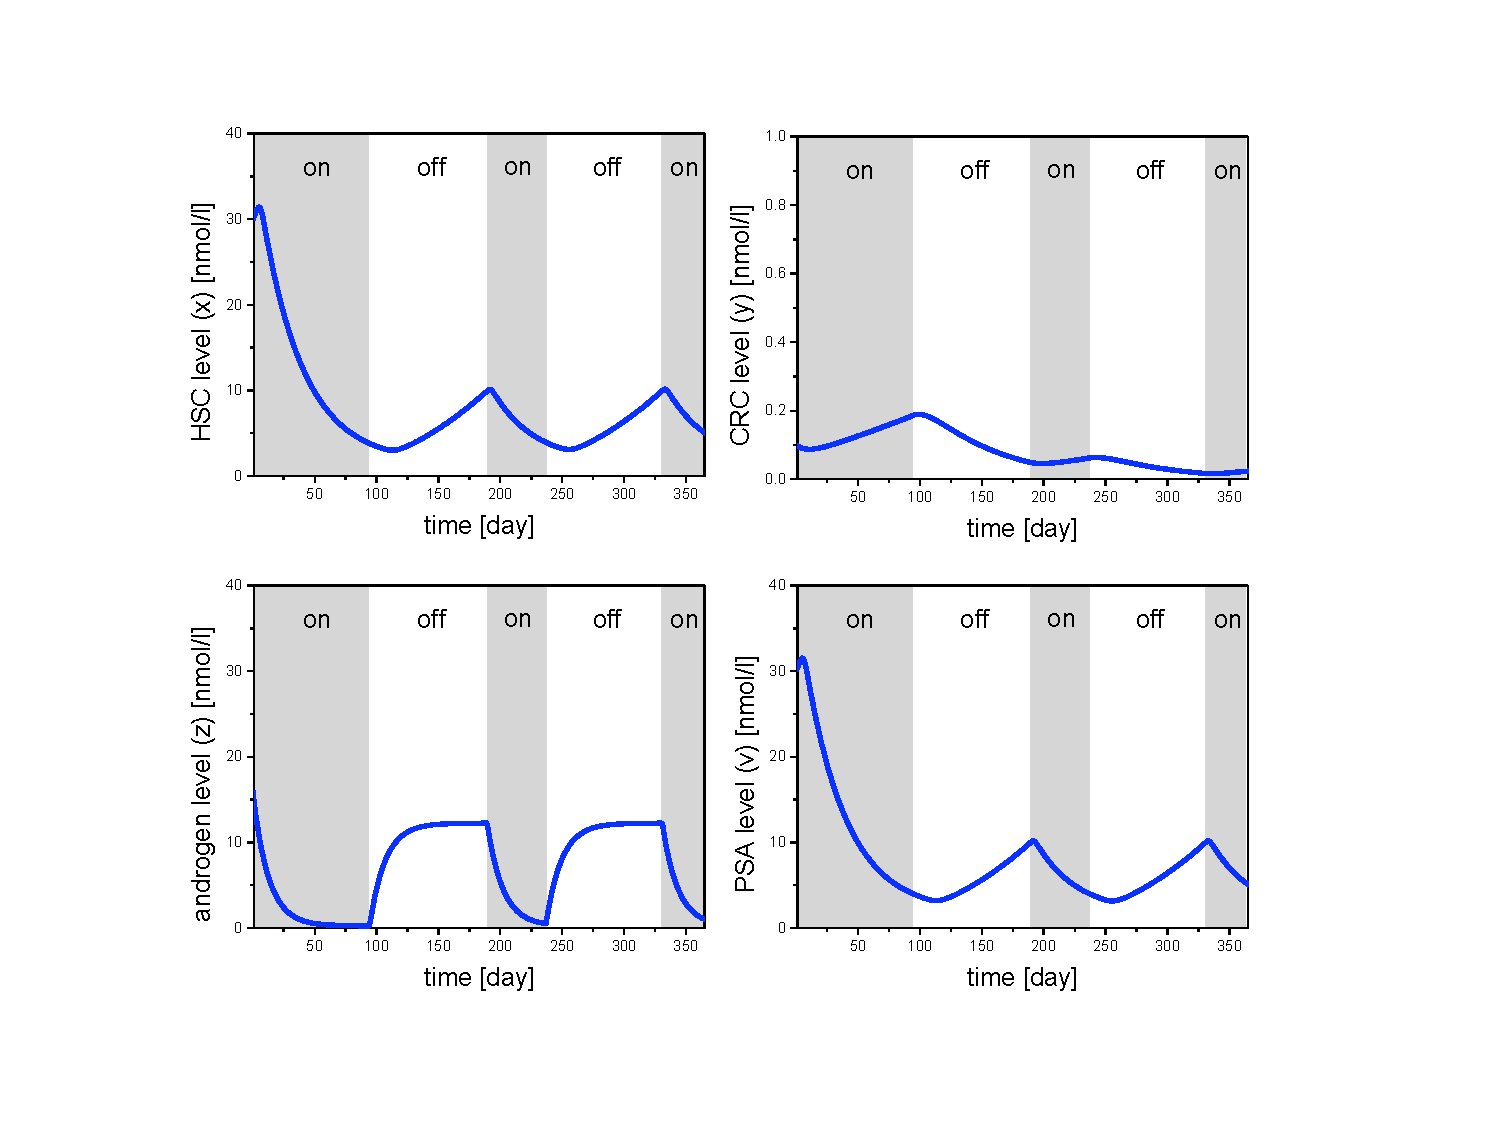
\includegraphics[scale=0.48]{fig-witness}
\caption{The simulated witness trajectories of the $H_3$ model.}
\label{prostate-fig1}
 %\vspace{-0.7cm}
\end{figure}

\subsection{Androgen-dependent HSC dynamics}

As mentioned in Section \ref{sec.model}, previous studies \cite{jackson04a,jackson04b,ideta08} modeled the androgen-dependent proliferation and apoptosis of HSCs using MML functions, while we use sigmoid functions. Here we show that the MML based approach is unable to reproduce an important dynamical property, but our model could. The patients' data in \cite{ bruchovsky06,bruchovsky07} show that the \textit{half-time} $t_{1/2}$ (i.e. the amount of time required for a quantity to fall to half its initial value) of PSA level under androgen suppression is often less than $60$ days. To specify this property, we introduced an auxiliary mode (Mode 3). If $v(t)=v(0)/2$, the system will jump from Mode 1 to Mode 3. Starting with Mode 1 and $20 \le x(0) \le 30$, we checked reachability of a goal state with $0 \le w \le 60$ for both Ideta's model \cite{ideta08} and our model. The results show that  $\delta$-$\mathsf{sat}$ was return for our model (Run\#4, Table \ref{runs}), while $\mathsf{unsat}$ was returned for Ideta's model (Run\#5, Table \ref{runs}), suggesting the superiority of sigmoid functions over MML functions in capturing HSC dynamics.


\begin{table}[!th]
  \centering
  \small
  \begin{tabular}{|c|c|c|c|c|}
    \hline
    \hline
    Run & Model & Initial State   & Result   & Time   \\
    \hline
    \hline
    1 & $H_1$ & $r_0 \in [0.0,7.99]$, $r_1 \in [8.0,15.0]$  & $\mathsf{unsat}$  &  3.94 \\
    2 & $H_2$ & $r_0 \in [0.0,7.99]$, $r_1 \in [8.0,15.0]$   & $\mathsf{unsat}$  &  5.26 \\
    3 & $H_3$ & $r_0 \in [0.0,7.99]$, $r_1 \in [8.0,15.0]$   & $\delta$-$\mathsf{sat}$ &  472 \\ 
    4 & $H_3$ & $x(0) \in [20.0,30.0]$   & $\delta$-$\mathsf{sat}$ &  10.1 \\
    5 & Ideta & $x(0) \in [20.0,30.0]$   & $\mathsf{unsat}$ &  0.5 \\           
    6 & $H_3$ & $r_0 \in [0.0,7.99]$, $r_1 \in [8.0,15.0]$   & $\delta$-$\mathsf{sat}$ &  526 \\ 
    7 & $H_3$ & $r_0 \in [0.0,7.99]$, $r_1 \in [8.0,15.0]$   & $\mathsf{unsat}$ &  0.3 \\ 
    8 & $H_3$ & $r_0 \in [0.0,7.99]$, $r_1 \in [8.0,15.0]$   & $\delta$-$\mathsf{sat}$ &  28 \\ 
    9 & $H_3$ & $r_0 \in [0.0,7.99]$, $r_1 \in [8.0,15.0]$   & $\delta$-$\mathsf{sat}$ & 203 \\ 
    \hline
    \hline
  \end{tabular}
  \caption{\small
  Experimental results.
    %\#Mode = Number of modes in the hybrid system,
    %\#Depth = Unrolling depth,
    %\#ODE = Number of ODEs in the unrolled formula,
    %Var = number of variables in the unrolled formula,
    Result = bounded model checking result,
    Time = CPU time (s),
    $\delta=10^{-3}$.
    %Trace = Size of the ODE trajectory
}\label{runs}
\end{table}
%}


\begin{table*}[t]
\caption{Estimated personalized parameters and suggested treatment schemes \label{prostate2}}
\centering
\small
\begin{tabular}{|c|c|c|c|c|}
\hline\hline
Parameter  & Patient\#1 & Patent\#11 & Patient \# 15 & Patient\#26  \\\hline\hline
$\alpha_x$ & 0.0204 d$^{-1}$ & 0.0204 d$^{-1}$ & 0.0213 d$^{-1}$& 0.0197 d$^{-1}$ \\
$\alpha_y$ & 0.0242 d$^{-1}$ &  0.0242 d$^{-1}$&  0.0242 d$^{-1}$&  0.0242 d$^{-1}$  \\
$\beta_x$  & 0.0201 d$^{-1}$ & 0.02 d$^{-1}$ & 0.01 d$^{-1}$& 0.0175 d$^{-1}$ \\
$\beta_y$  & 0.0168 d$^{-1}$ &0.0158 d$^{-1}$ &0.0168 d$^{-1}$ &0.0168 d$^{-1}$  \\
$k_1$     & 10.0 nM & 7.0 nM & 7.0 nM& 10.0 nM  \\
$k_2$     & 1.0 & 1.0 & 1.0 & 1.0 \\
$k_3$     & 10.0 nM & 7.0 nM & 7.4 nM& 10.0 nM  \\
$k_4$     &  2 & 2 & 2 & 2   \\
$m_1$     & 0.00005 d$^{-1}$ &  0.00005 d$^{-1}$ &  0.00005 d$^{-1}$ &  0.00005 d$^{-1}$  \\
$z_0$     & 12.0 nM & 9.0 nM & 8.0 nM & 12.0 nM  \\
$\tau$     & 12.5 d & 12.5 d & 12.5 d & 12.5 d  \\
$\lambda_x$     & 0.01 d$^{-1}$ & 0.0121 d$^{-1}$ & 0.01 d$^{-1}$ & 0.01 d$^{-1}$ \\
$\mu_x$     & 0.05 d$^{-1}$ & 0.06 d$^{-1}$ & 0.02 d$^{-1}$ & 0.03 d$^{-1}$\\
$\mu_z$     & 0.02 d$^{-1}$ & 0.02 d$^{-1}$  & 0.02 d$^{-1}$ & 0.02 d$^{-1}$  \\
\hline\hline
Scheme     & $r_0=5.2$, $r_1=10.8$ & N.A & $r_0=1.9$, $r_1=8.0$ & $r_0=4.6$, $r_1=10.7$ \\
\hline\hline
\end{tabular}
 %\vspace{-0.7cm}
\end{table*}



\subsection{Personalized therapy design}
We next apply $\delta$-reachability analysis to design treatment schemes for individual patients. The parameter values shown in Table \ref{prostate} were estimated by fitting the data of Patient\#1. As Patient\#1 has typical response kinetics to IAS, we treated these values as the baseline parameters. As we demonstrated in Figure \ref{data}, the values of some parameters vary among patients. Such variability may significantly affect the hormone therapy responses. 
%
%We select a set of ``personalized parameters'' including $\alpha_x$ (the proliferation rate of HSCs), $\beta_x$ (the apoptosis rate of HSC cell), $m_1$ (the conversion rate from HSCs to CRCs), and $z(0)$ (normal androgen level). 
%
%The values of these parameters can be either experimentally measured \citep{berges95} or computationally determined from PSA time serials data \citep{hirata10}.
%
For example, Figure \ref{patients}(a-c) illustrates the PSA dynamics of $3$ mock patients with different personalized parameters under the same IAS treatment scheme ($r_0=4$, $r_1=10$). IAS prevents the relapse for Patient A and delays the relapse for Patient B, but does not help Patient C. Figure \ref{patients}(d) shows that, by modifying the IAS scheduling parameters $r_0$ and $r_1$, the relapse of Patient C can be avoided or delayed. 

\begin{figure}[htb]
\centering
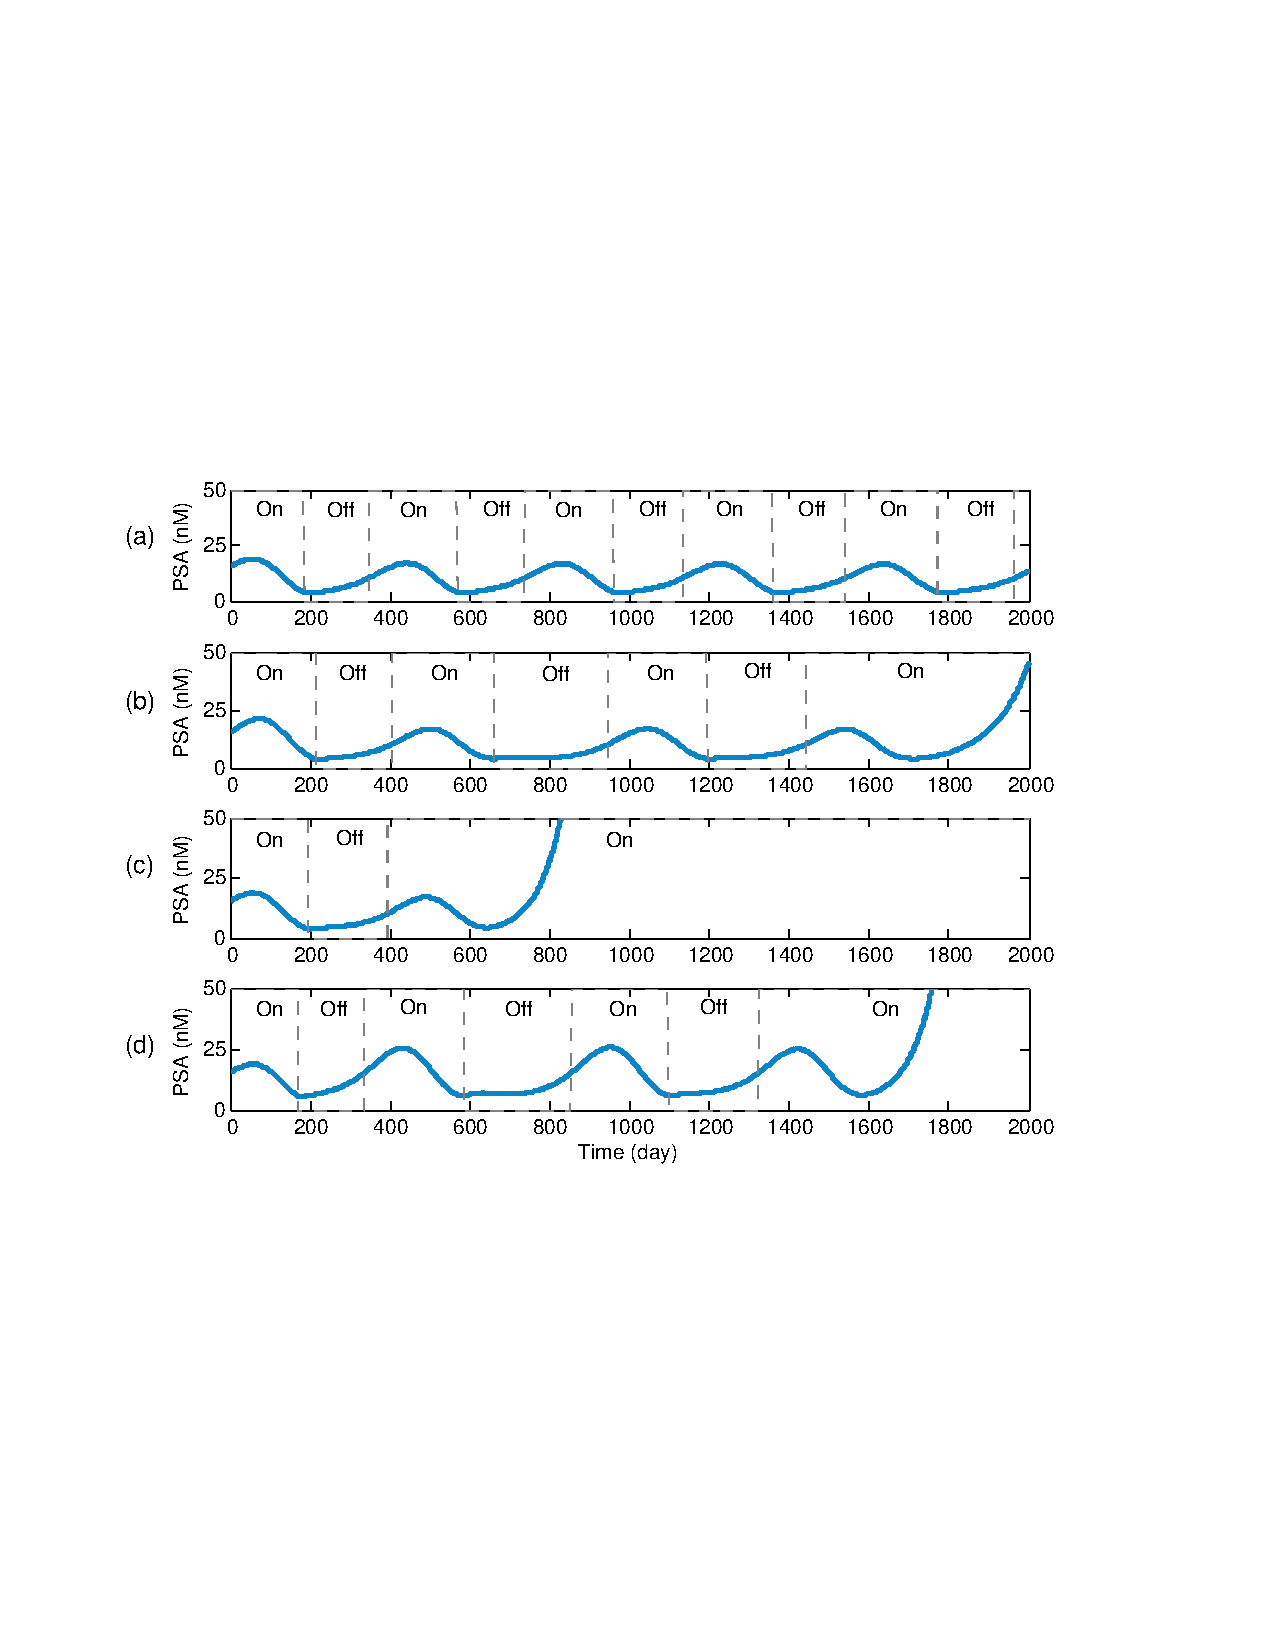
\includegraphics[scale=0.52]{fig-prostatetraj2}
\caption{Simulated PSA profiles of patients with different parameters. (a) Patient A: $\alpha_y=0.0242$, $\beta_y=0.0168$, $m_1=0.00005$, $z(0)=12$, $r_0=4$, $r_1=10$ (b) Patient B: $\alpha_y=0.24$, $\beta_y=0.13$, $z(0)=13$, $m_1=0.0001$, $r_0=4$, $r_1=10$ (c) Patient C: $\alpha_y=0.35$, $\beta_y=0.187$, $m_1=0.00005$, $z(0)=10$, $r_0=4$, $r_1=10$ (d) Patient C: $\alpha_y=0.035$, $\beta_y=0.187$, $m_1=0.00005$, $z(0)=10$, $r_0=6$, $r_1=15$.}
\label{patients}
 %\vspace{-0.7cm}
\end{figure}

Given the personalized parameters of a individual patient, we can design a treatment scheme for him that might avoid cancer relapse with bounded time by solving the following parameter identification problem: (i) set the ranges of scheduling parameters as $r_0 \in [0,7.99]$ (nM) and $r_1 \in [8,15]$; (ii) check if $H_3$ can reach the goal state without violating the ``no cancer relapse'' invariants within $1$ year. If $\mathsf{unsat}$ was returned, it means that androgen suppression therapy is not suitable for the patient. The patient has to resort to other kinds of therapeutic interventions. Otherwise, when the $\delta$-$\mathsf{sat}$ answer is returned, a treatment scheme containing feasible values of $r_0$ and $r_1$ will also be returned, which could help preventing or delaying the relapse within bounded time. Note that if $r_0=0$ is returned, it implies that the CAS scheme, instead of IAS scheme, might be more suitable for the patient.

The personalized parameters of individual patients can be obtained by collectively fitting the available experimental data. %We adapted stochastic ranking evolutionary strategy (SRES) \cite{sres}, a standard global optimization method, to explore the high-dimentional parameter space. 
%Recent studies \cite{leder14,sorger12} showed that cancer therapy might change the patient state and lead to different therapeutic responses. Thus, we propose an adaptive control based framework. The underlying assumption is that
%
We tested our method on real patients data collected by \cite{bruchovsky07}. The parameter values for each selected patient were estimated by fitting the model to the PSA time serials data under the IAS therapy\footnote{Data available at \url{http://www.nicholasbruchovsky.com/clinicalResearch.html}.}. As an example, Figure \ref{fitting} shows the comparison between model predictions and the experimental data of PSA and androgen levels for Patient\#1, Patient\#11, Patient\#15, and Patient\#26. Table \ref{prostate2} summarized the suggested treatment scheme we obtained using $\delta$-reachability analysis (Run\#6-9, Table \ref{runs}). Note that for Patient\#11, $\mathsf{unsat}$ was returned, implying that no suitable treatment schemes were identified.

%Show witness graphs? 

\begin{figure}[htb]
\centering
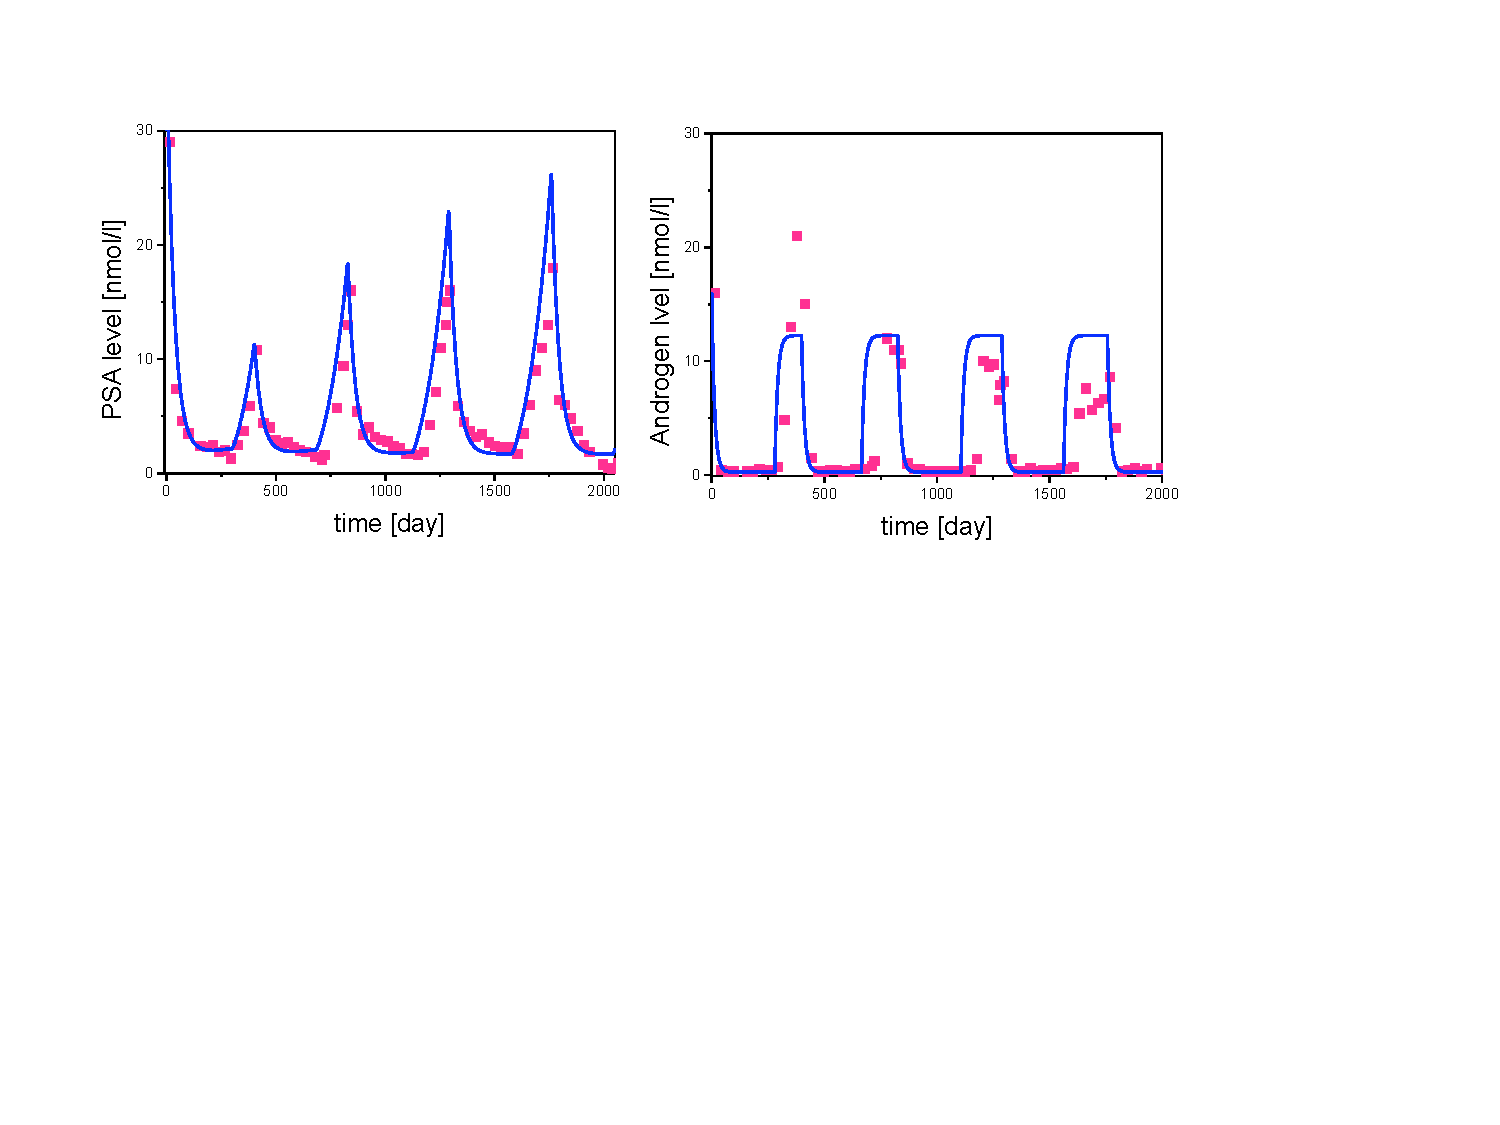
\includegraphics[scale=0.48]{fig-fitting}
\caption{Model prediction vs. experimental data.}
\label{fitting}
%\vspace{-0.7cm}
\end{figure}


